\question{} 

La méthode read lit un caractère depuis la position courante, renvoie une chaine.

La méthode readline lit le reste de la ligne depuis la position courante, renvoie une chaine.

La méthode readlines lit toutes les lignes depuis la position courante, renvoie une liste de chaines.

\question{} 


Ce sont les caractères \og tabulation\fg{} et \og nouvelle ligne\fg{} .


\question{}

\begin{pyverbatim}
def carac(nom_de_fichier):
    """Renvoie une liste contenant le nombre de caractères 
       de chaque ligne de nom_de_fichier"""
    with open(nom_de_fichier,'r',) as f:
        lignes = f.readlines()
    return [len(x.strip('\n')) for x in lignes]
\end{pyverbatim}

\question{}
\begin{lstlisting}
def compte_carac(carac,nom_de_fichier):
    with open(nom_de_fichier,'r',encoding='utf8') as f:
        ligne='_'
        S=0
        while ligne!='':
            ligne = f.readline().lower()
            for c in ligne:
                if c==carac.lower():
                    S+=1
        return S
\end{lstlisting}

\begin{lstlisting}
def compte_carac2(carac,nom_de_fichier):
    with open(nom_de_fichier,'r',encoding='utf8') as f:
        texte=f.read()
        return texte.lower().count(carac)
\end{lstlisting}


\question{}

\begin{lstlisting}
def stat_carac(nom_de_fichier):
    alphabet='abcdefghijklmnopqrstuvwxyz'
    occurences=[]
    for car in alphabet:
        occurences.append(compte_carac(car,nom_de_fichier))
    return occurences
\end{lstlisting}


\question{}

Il faut importer ces modules et fonctions : 
\begin{lstlisting}
import matplotlib.pyplot as plt
from numpy import arange
\end{lstlisting}

\begin{minipage}{0.5\textwidth}
\textbf{Méthode 1 : graphe}

\begin{lstlisting}
def trace_stat_carac(nom_de_fichier):
    y=stat_carac(nom_de_fichier)
    plt.clf()
    plt.plot(y,'ro')
    plt.xlabel("Numéro de la lettre dans l'alphabet")
    plt.ylabel('occurences')
    plt.savefig('graphe_occurences.png')
\end{lstlisting}

\end{minipage}
\begin{minipage}{0.5\textwidth}
\begin{center}
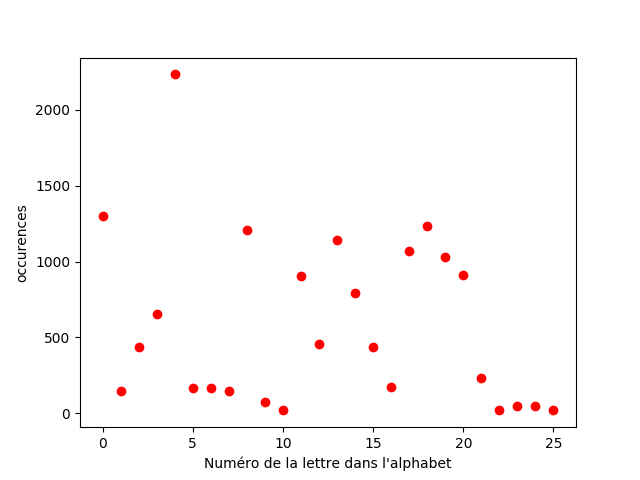
\includegraphics[width=0.9\textwidth]{graphe_occurences.png}
\end{center}
\end{minipage}

\begin{minipage}{0.5\textwidth}
\textbf{Méthode 2 : histogramme}

\begin{lstlisting}
alphabet='abcdefghijklmnopqrstuvwxyz'
alphabet_liste=len(alphabet)*[]
for c in alphabet:
    alphabet_liste.append(c)
def trace_stat_carac_bis(nom_de_fichier):
    y=stat_carac(nom_de_fichier)
    plt.clf()
    for i,yi in enumerate(y):
        plt.plot([i,i],[0,yi],'r-',linewidth=5)
    plt.ylabel('occurences')
    plt.xticks(arange(26),tuple(alphabet_liste))
    plt.savefig('histo_occurences.png')
    plt.show()
\end{lstlisting}

\end{minipage}
\begin{minipage}{0.5\textwidth}
\begin{center}
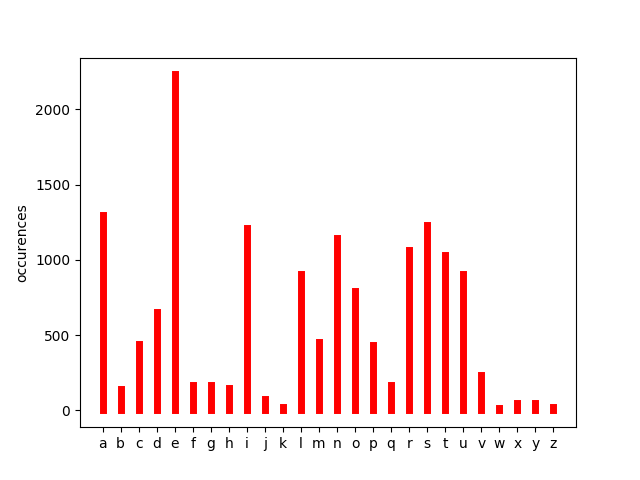
\includegraphics[width=0.9\textwidth]{histo_occurences.png}
\end{center}
\end{minipage}
